\documentclass[tikz, border=10pt]{standalone}
\usetikzlibrary{decorations.pathreplacing, calligraphy}

\begin{document}
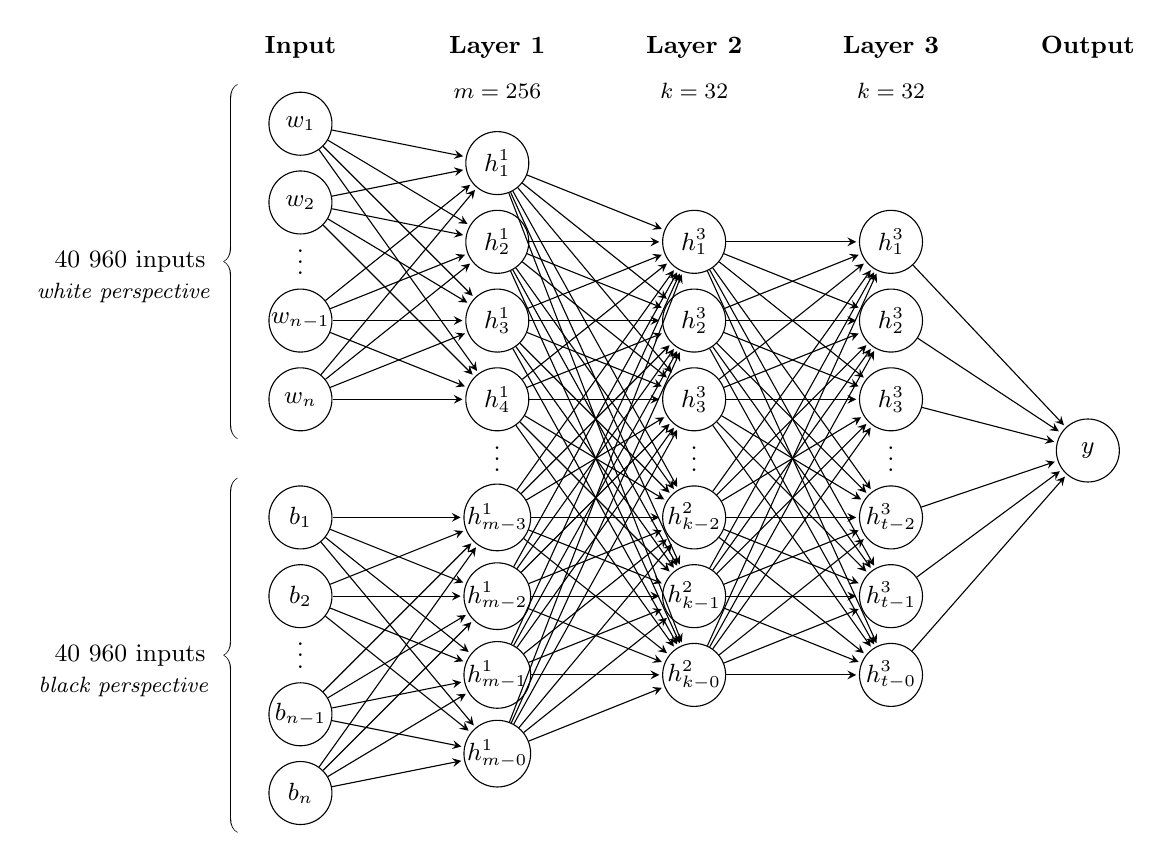
\begin{tikzpicture}[
    neuron/.style={circle, draw, minimum size=0.8cm, inner sep=0pt},
    connector/.style={-stealth, thin, shorten >=1pt},
    % Style pour l'accolade académique
    mybrace/.style={decorate, decoration={calligraphic brace,mirror, amplitude=5pt}}
]
\tikzstyle{every node}=[font=\small]



% --- COUCHE D'ENTRÉE ---
% Whites
% Neurones du haut
\node[neuron, ] (in-w1) at (0,0) {$w_1$};
\node[neuron] (in-w2) at (0,-1.0) {$w_2$};

% Points de suspension au milieu
\node at (0,-1.65) {$\vdots$};

% Neurones du bas
\node[neuron] (in-wn1) at (0,-2.5) {$w_{n-1}$};
\node[neuron] (in-wn) at (0,-3.5) {$w_n$};

% blacks
% Neurones du haut
\node[neuron, ] (in-b1) at (0,-5.0) {$b_1$};
\node[neuron] (in-b2) at (0,-6.0) {$b_2$};

% Points de suspension au milieu
\node at (0,-6.65) {$\vdots$};

% Neurones du bas
\node[neuron] (in-bn1) at (0,-7.5) {$b_{n-1}$};
\node[neuron] (in-bn) at (0,-8.5) {$b_n$};




% --- ACCOLADE ---
\draw[mybrace] (-0.8, 0.5) -- (-0.8, -4.0) 
    node[midway, left=8pt, font=\small] {40 960 inputs};

\draw[mybrace] (-0.8, -4.5) -- (-0.8, -9.0) 
    node[midway, left=8pt, font=\small] {40 960 inputs};

% --- COUCHE CACHÉE 1 ---
\foreach \j in {1,...,4}
    \node[neuron] (h1-\j) at (2.5, -\j*1.0 + 0.5) {$h^1_\j$};
    
\node at (2.5, -4.15) {$\vdots$};

\foreach \j [evaluate=\j as \jj using {int(8 - \j)}] in {5,...,8}
    \node[neuron] (h1-\j) at (2.5, -\j*1.0 ) {$h^1_{m-{\jj}}$};

% --- COUCHE CACHÉE 2 ---
\foreach \j in {1,...,3}
    \node[neuron] (h2-\j) at (5.0, -\j*1.0 - 0.5) {$h^3_\j$};
    
\node at (5.0, -4.15) {$\vdots$};

\foreach \j [evaluate=\j as \jj using {int(6 - \j)}] in {4,...,6}
    \node[neuron] (h2-\j) at (5.0, -\j*1.0 - 1.0 ) {$h^2_{k-{\jj}}$};

% --- COUCHE CACHÉE 3 ---
\foreach \j in {1,...,3}
    \node[neuron] (h3-\j) at (7.5, -\j*1.0 - 0.5) {$h^3_\j$};
    
\node at (7.5, -4.15) {$\vdots$};

\foreach \j [evaluate=\j as \jj using {int(6 - \j)}] in {4,...,6}
    \node[neuron] (h3-\j) at (7.5, -\j*1.0 - 1.0 ) {$h^3_{t-{\jj}}$};

% --- COUCHE DE SORTIE ---
\node[neuron] (out) at (10, -4.15) {$y$};

% --- CONNEXIONS (Épurées) ---
% On connecte seulement quelques neurones pour ne pas surcharger le dessin
\foreach \i in {w1,w2,wn1,wn}
    \foreach \j in {1,2,3,4}
        \draw[connector] (in-\i) -- (h1-\j);

\foreach \i in {b1,b2,bn1,bn}
    \foreach \j in {5,...,8}
        \draw[connector] (in-\i) -- (h1-\j);


\foreach \i in {1,...,8}
    \foreach \j in {1,...,6}
        \draw[connector] (h1-\i) -- (h2-\j);

\foreach \i in {1,...,6}
    \foreach \j in {1,...,6}
        \draw[connector] (h2-\i) -- (h3-\j);
% \foreach \i in {5,...,8}
%     \foreach \j in {4,...,6}
%         \draw[connector] (h1-\i) -- (h2-\j);
        
\foreach \j in {1,...,6}
    \draw[connector] (h3-\j) -- (out);

% --- LABELS DE DIMENSION (La partie qui t'intéresse) ---
% On définit une hauteur fixe Y=1.2 pour l'alignement
\node[above, font=\bfseries\small] at (0, 0.7) {Input};
\node[above, font=\bfseries\small] at (2.5, 0.7) {Layer 1};
\node[above, font=\bfseries\small] at (5.0, 0.7) {Layer 2};
\node[above, font=\bfseries\small] at (7.5, 0.7) {Layer 3};
\node[above, font=\bfseries\small] at (10.0, 0.7) {Output};

% Les valeurs numériques (en italique mathématique)
\node[above, font=\itshape\footnotesize] at (2.5, 0.2) {$m=256$};
\node[above, font=\itshape\footnotesize] at (5.0, 0.2) {$k=32$};
\node[above, font=\itshape\footnotesize] at (7.5, 0.2) {$k=32$};
% \node[above, font=\itshape\footnotesize] at (9.0.0, -0.8) {$k=32$};
\node[above, font=\itshape\footnotesize] at (-2.25, -2.40) {white perspective};
\node[above, font=\itshape\footnotesize] at (-2.25, -7.40) {black perspective};



\end{tikzpicture}
\end{document}